\documentclass[../main.tex]{subfiles}

\begin{document}

\chapter{Overview of potential solutions}

This chapter theoretically elaborates on different approaches to implementing the requirements defined in chapter \ref{requirements}.
The sketched protocols in the following sections illustrate different encryption techniques.
Each section details the consequences of the technique to the requirements of this thesis.
The outcome of this chapter is a set of possible solution strategies.

\section{External encryption}
\label{sec:external-encryption}
An intuitive way of implementing a protocol that allows the exchange of logs among users is to rely on external encryption tools.
Suppose that Alice wants to share a log with Bob.
Alice could send the log to Bob with an encrypted email.
Emails can be encrypted with dedicated protocols, e.g. PGP~\footnote{Defined by IETF in \href{https://www.rfc-editor.org/rfc/rfc4880}{RFC4800}.} or S/MIME~\footnote{Defined by IETF in \href{https://www.rfc-editor.org/rfc/rfc8551.html}{RFC8551}.}.
Such encryption technologies allow Alice to confidentially share logs with others.
This approach, however, is limited and does not satisfy the identified requirements.
It is the responsibility of the user to correctly apply the protocol.
This is error-prone, it could lead to unintended security issues and it is not user-friendly.
Sharing the log with $n$ users requires Alice to send $n$ encrypted emails.
More importantly, this approach does not end-to-end encrypt logs because the server storing the logs still has access to the unencrypted data.
Since the Overseer server is not trusted, confidentiality is broken (security requirement S1).
Once an encrypted email is sent to the receiver there is no way for Alice to revoke any access to the log.
She loses control over the encrypted log because Bobs' email provider stores the cipher.
This is not in the control of the toolchain.
This implies, that Alice can not revoke the access anymore (functional requirement F3).
Those limitations motivate the implementation of a more sophisticated protocol.

\section{Mutual encryption}
\label{sec:mutual-encryption}
The term mutual encryption refers to the idea that logs are encrypted mutually between users in the system.
If each user is assigned a key pair, a data owner can encrypt a log for each user separately.
The core idea is similar to the approach presented for external encryption (section \ref{sec:external-encryption}).
However, this approach integrates the encryption and decryption of logs into the toolchain.
To better understand this approach consider the following example.
A monitor component accesses data of Alice and therefore creates a log.
Since Alice needs to be able to access the log, the monitor encrypts the log under the public key of Alice and sends it to the server.
If Alice keeps her secret key private she is the only entity who can decrypt the log.
She can download the log, decrypt it, and also share it with Bob by re-encrypting it under his public key.
The re-encrypted data is then sent to the server where it is stored.
Bob can finally download and decrypt the shared log.

Alice can access the log because the monitor encrypted it with her public key.
She can also share logs with others.
The encrypted data is stored by the Overseer server.
It allows Alice to request the deletion of the cipher from the server.
This way Alice can revoke access to the log.
Thus, all functional requirements are fulfilled.
As long as all users have exclusive access to their secret key, this approach also ensures the confidentiality of the log (security requirement S1).
To defend against malicious data owners creating forged logs, the monitor component (e.g. the entity creating a log) needs to cryptographically sign the log before encryption.
If Alice shares the log, she does not share the plain log.
Rather, she encrypts the signed log.
Alice can not modify the existing log or create a completely new log because she is not able to compute a valid signature in the name of the monitor.
She could only succeed by knowing the secret key of the monitor.
This structure allows the receiver to verify if the log was created by a valid monitor component.
As a consequence, a forged log can be detected during decryption (security requirement S3).
Security requirement S2 can also be satisfied.
To achieve this, Alice does not only encrypt the signed log.
She additionally signs and includes the identity of the receiving user.
This allows receivers to verify if the log was intended for them.
Figure \ref{fig:mutual_encryption} shows the structure of a log before it is encrypted.
The actual access log is signed by the monitor.
The shared log is a data structure that contains the signed access log.
It additionally specifies the user with whom the log is shared (e.g. receiver).
The shared log itself is signed by the data owner.
The signed share log is passed to the encryption algorithm.
After decryption, a receiver can validate if the sender intentionally shared the log.
The receiver can also verify if the nested access log was signed by the claimed monitor.

\begin{figure}[ht]
    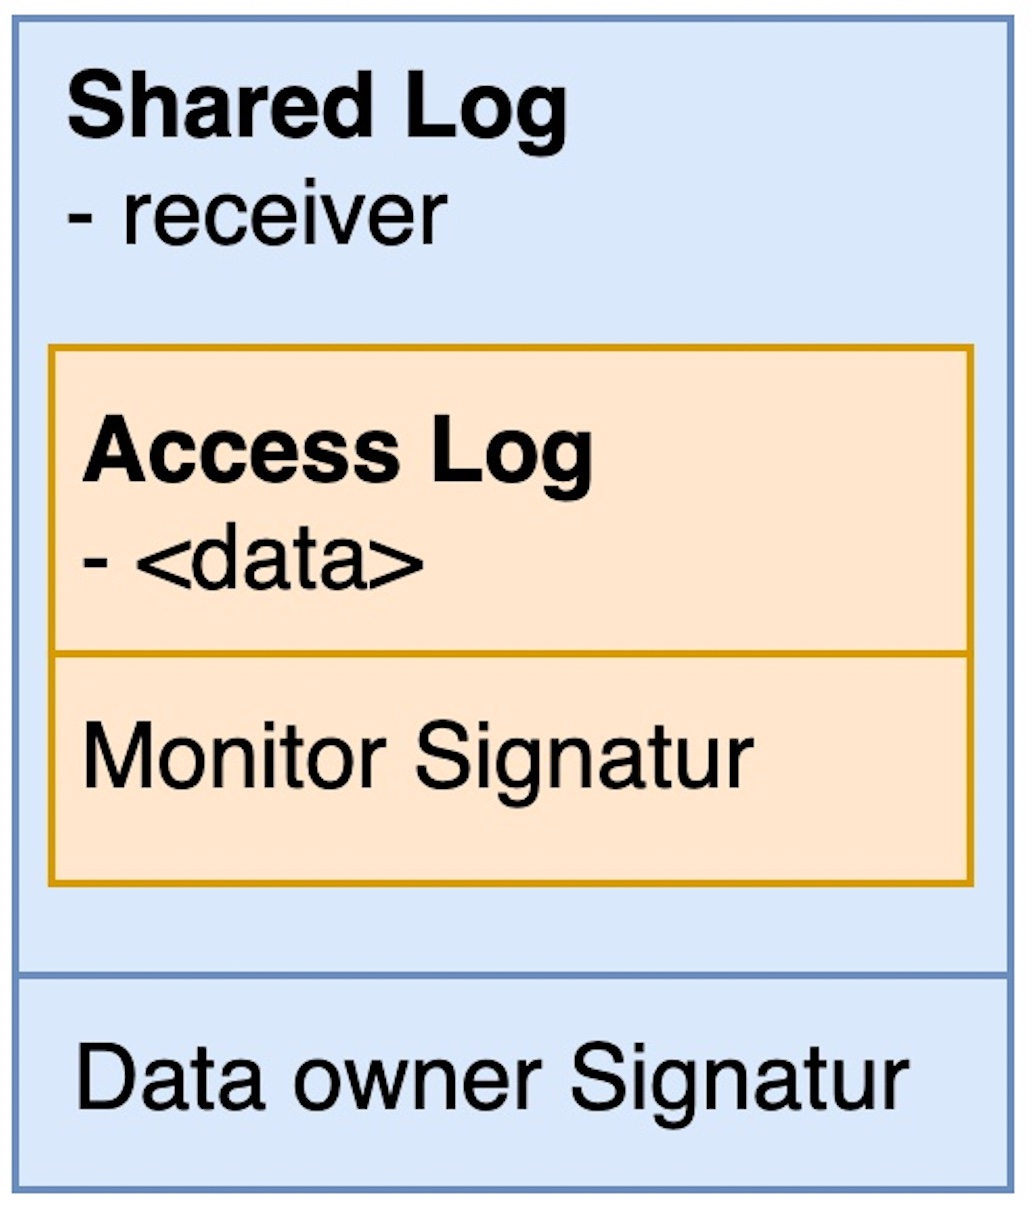
\includegraphics[scale=0.12]{../img/04/mutual_encryption.jpg}
    \centering
    \caption{Structure of a shared log before encryption.}
    \label{fig:mutual_encryption}
\end{figure}

While this approach fulfills all functional and security requirements it suffers from performance problems.
Similar to external encryption, the whole log needs to be encrypted $n$ times if it is shared with $n$ users.
Much more problematic, however, is the application of asymmetric cryptography to application data.
Public-key cryptography relies on intense mathematical computations and should not be used to encrypt large amounts of data directly~\cite[340]{Eckert2018}.
Eckert justifies this with the fact that asymmetric encryption algorithms are muss less performant than symmetric algorithms.
Following her argumentation, asymmetric cryptography is therefore usually used to encrypt a symmetric key which finally encrypts the larger payload.
Thus, the implemented protocol should avoid the encryption of log data with asymmetric algorithms.

\section{Key server}
\label{sec:key-server}
The development of cloud computing and centralized software architectures motivated the idea of key servers~\cite{Seitz2003}.
A key server stores cryptographic keys on behalf of the user.
If a user authenticates against the server and has the required permissions it can access a particular key.
This can be useful in environments where multiple users need to access the same key.
The creator and owner of a key can upload the key to the key server.
If others require access to the key, the owner can modify the access policy.

The concept of a key server can also be applied to share encrypted logs.
Once a monitor creates a log because it accesses sensitive data of Alice, the monitor creates a symmetric key and encrypts the log under this symmetric key.
The encrypted log is sent to the Overseer.
To decrypt the log, Alice requires access to this symmetric key.
Thus, the monitor needs to upload the generated key to the key server which allows Alice to download it.
If she wants to share the log with Bob, there is no need to re-encrypt any data in the Overseer.
Rather, she needs to tell the key server that Bob is allowed to access this key.
Alice can also revoke any access to the file.
She could simply tell the key server that a particular user is not allowed to access the key anymore.
However, if a malicious user stored the key on his local machine, the revocation does not have any effect.
It is better to additionally re-encrypt the encrypted log in the Overseer with a freshly generated key, which is then also uploaded to the key server.

This example shows that all functional requirements can be satisfied when utilizing a key server.
The techniques introduced in section \ref{sec:mutual-encryption} to satisfy security requirements S2 (sign the receiver of the shared log) and S3 (sign the access log) can be applied here, too.
Security requirement S1, however, can not be met because the administrator of the key server has access to all keys.
The confidentiality of all logs is broken because this allows him to potentially decrypt all logs.
In section \ref{sec:end-to-end} it became clear that the encryption endpoints in E2EE systems can be defined arbitrarily.
The here sketched protocol can nevertheless be classified as E2EE if the key server is defined as a valid decryption endpoint.
But this does not meet the intuitive understanding of E2EE.
The utilization of a key server also implies that we require an additional trusted component.
This increases the attack surface of the system and does not adhere to the non-functional requirement N1 (minimal number of trusted entities).

\section{Attribute-based encryption}

Attribute-based encryption is an approach to provide access control within the domain of cryptography~\cite{Bethencourt2007}. 
Without attribute-based encryption, access control techniques need to be implemented by a server. 
Access will be granted if the requesting user is allowed to read/write the data (e.g. if the user works for a certain company). 
Thus, the server ensures that only authorized entities access data. 
Consider the case where this server is compromised: 
The attacker has unlimited access to the stored data because the access control techniques are no longer in place and the data itself is not encrypted.
Attribute-based encryption schemes shift the logic of access control into encryption and decryption algorithms. 
A distinction is made between a set of possible attributes (e.g. ${A,B,C}$) and a policy. 
Policies are logical expressions over attributes (e.g. $A \land B \land \neg C$). 
A secret key of a user contains certain attributes. 
During encryption, a user specifies a policy that is encoded into the ciphertext.
A ciphertext can only be decrypted with a secret key fulfilling that policy.
Within the domain of \textit{ABE}, one can differentiate between \textit{ciphertext-policy ABE} and \textit{key-policy ABE}. 
The above-described scenario, where the policy is encoded into the ciphertext and the key of the user is checked against this policy is called \textit{ciphertext-policy ABE}. 
On the contrary, \textit{key-policy ABE} describes the scenario, where the policy is encoded into the key of the user.
Thus, a user can only decrypt a ciphertext that is annotated with the corresponding attributes.~\cite{Bethencourt2007}

The notation of \textit{ciphertext-policy ABE} directly can be used to encrypt data for multiple receivers. 
During encryption, a policy is defined. 
All users which are equipped with attributes fulfilling this policy can decrypt data.
By encoding the name of the valid receivers into the policy, the encrypting user could specify the set of users who can decrypt.
If the access of a user needs to be revoked, the cipher is re-encrypted with a new set of receivers.
This ensures that all required functional requirements are met.
One can equip the logs with cryptographic signatures (as described in section \ref{sec:mutual-encryption}).
This technique fulfills the security requirements S2 (the receiver can verify it is a valid encryption endpoint) and S3 (the data owner can not forge logs).

Attribute-based encryption usually relies on a trusted key generation center~\cite{Sahai2009}.
It computes and distributes cryptographic keys.
This implies key escrow and harms security requirement S1 because the trusted server can potentially decrypt all ciphers.
Additionally, each trusted entity increases the attack surface of the toolchain and conflicts with the non-functional requirement N1 (minimal number of trusted entities).
There are also schemes that avoid a centralized trust center by employing a decentralized architecture~\cite{Vaanchig2018}.
These systems, however, can not be integrated into the centralized architecture of the existing toolchain.

\section{Broadcast encryption}
The notation of broadcast encryption (\textit{BE}) was first introduced by~\citeauthor{fiat1993broadcast}~\cite{fiat1993broadcast}. 
Since then many different approaches to broadcast encryption schemes were proposed. 
All of them solve the following challenge: 
How to broadcast encrypted data while only an explicitly defined set of users can decrypt the data?
This section introduces different approaches to realize broadcast encryption.


\subsection{Identity-based broadcast encryption} 
Identity-based broadcast encryption schemes (\textit{IBBE}) are the result of merging identity-based encryption (\textit{IBE}) with broadcast encryption techniques (\textit{BE})~\cite{Sakai2007}.
\textit{IBE} was initially taken into consideration by Shamir in 1985~\cite{shamir1985}.
It is public-key cryptography where the public key of a user is a unique string, e.g. its email address. 
Secret keys are derived from this unique string via a dedicated derivation function. 
To compute secret keys, identity-based encryption schemes require a trusted third party that computes and distributes secret keys for each user.
Otherwise, everyone could compute the secret key of arbitrary users resulting in an inherent insecure public-key cryptography scheme.
Identity-based cryptography was later combined with broadcast encryption resulting in \textit{IBBE}~\cite{Sakai2007}.
In these systems, a message can be encrypted for a dedicated set of users, where each user is identified by a unique string.
The encryption algorithm requires a plaintext and a set of identities~\cite{shamir1985}.
Decryption requires the secret key of one of the users specified during encryption.

Suppose that Alice wants to share encrypted data with Bob.
One Alice and Bob received their secret keys from the trust center, Alice can encrypt the log and specify Bob as a valid receiver.
She can then upload the cipher.
Bob can download and decrypt using his secret key.
If Alice wants to revoke access of Bob, she needs to re-encrypt the cipher and upload it again.
Thus, all three functional requirements can be fulfilled.
The techniques from section \ref{sec:mutual-encryption} can be applied, too.
This satisfies the security requirements S2 (the receiver can verify it is a valid encryption endpoint) and S3 (the data owner can not forge logs).

\textit{IBBE} schemes suffer from key escrow because a trusted party computes and distributes secret keys.
The additional trusted entity increases the attack surface.
Moreover, key escrow harms the notation of E2EE because the key generation server could potentially decrypt all ciphers.

\subsection{Certificate-based broadcast encryption}
Certificate-based encryption (\textit{CBE}) was introduced by \citeauthor{Gentry2003} in 2003~\cite{Gentry2003}. 
Later, this idea was adopted with broadcast encryption by allowing multiple receivers~\cite{Li2018, Fan2013}.
The construction of \textit{CBE} schemes is motivated by the following observations~\cite{Gentry2003}:

\begin{itemize}
    \item Classical public key encryption (\textit{PKE}) schemes suffer from the certificate revocation problem (detail in \cref{terms}).
    \item Identity-based encryption schemes suffer from key escrow (details in \cref{IBBE}).
    However, since they make use of implicit certification (details in \cref{IBBE}), \textit{IBE} schemes do not suffer from the certificate revocation problem.
    \item Combining both techniques -- \textit{PKE} and \textit{IBE} -- yields the new construction \textit{CBE}. 
    It neither suffers from key escrow nor from the certificate revocation problem.
\end{itemize}

Consider the scenario where Alice wants to send encrypted data to Bob. 
According to~\cite{Gentry2003}, \textit{CBE} schemes function as followed\footnote{For the sake of reduced complexity this is a simplified description.}:

\begin{enumerate}
    \item Alice generates a key pair with a \textit{PKE} key generation algorithm. She keeps the secret key secret. 
    Not even the trust center is allowed to know this secret key.
    \item Alice requests a certificate for her public key. 
    This certificate is created by the trust center by executing the \textit{IBE} key generation algorithm. 
    Thus, this certificate can technically also be seen as the second secret key of Alice, which the trust center knows.
    \item Bob also executes steps 1 and 2.
    \item To encrypt data for Bob, Alice uses Bobs public key and encrypts the message twice: Once, with the \textit{IBE} encryption algorithm and once with the \textit{PKE} encryption algorithm. The doubly encrypted message is then sent to Bob. In particular, there is no need for Alice to check if Bob has a valid certificate. This avoids the certificate revocation problem.
    \item Upon receiving the encrypted message, Bob needs to double decrypt the cipher. 
    Once, with the \textit{IBE} decryption algorithm and once with the \textit{PKE} decryption algorithm. 
    This enforces the following.
    First, only Bob can apply the \textit{PKE} decryption, because only he knows the required secret key. 
    Second, Bob needs a valid certificate because otherwise, he could not apply the \textit{IBE} decryption. 
    In particular, the first fact avoids key escrow (because the trust center does not know the secret key of Bob) and the second fact avoids the certificate revocation problem (because Bob can only decrypt with a valid certificate).
\end{enumerate}

This idea was later adopted to broadcast encryption.
The construction yields a certificate-based broadcast encryption scheme (\textit{CBBE})~\cite{Li2018}.
Although this construction relies on a key generation center it does not suffer from key escrow.
Once keys are established, a user can encrypt data for a dedicated set of users.
Only these users can decrypt the cipher.
In particular, the key generation center can not decrypt the cipher because it does not have access to the PKE secret key of a user.
Besides the functional requirements, \textit{CBBE} also satisfies the security requirements.
The separation of shared log and signed log introduced in section \ref{sec:mutual-encryption} can be applied.
Thus, all receivers can validate that they are intended decryption endpoints and that the access log was created by the claimed monitor.
The notion of E2EE is also fulfilled because the trusted server can not decrypt.

Unfortunately, no reference implementations of \textit{CBBE} exist. 
This fact is a major drawback in the context of this thesis.
These cryptographic systems are currently the subject of research.
There are no ongoing standardization processes to analyze their security.
As a result, the non-functional requirement N2 (standardized cryptographic algorithms) can not be met.
Using those schemes in a practical implementation is avoided in this thesis because the missing standards introduce an unpredictable risk.

\subsection{Proxy re-encryption based broadcast encryption}
Broadcast encryption schemes can be implemented with a technique named proxy re-encryption (\textit{PRE}).
Proxy re-encryption systems are cryptographic schemes, in which a third party (a.k.a. a \textit{proxy}) converts a ciphertext, which was originally intended for Alice, to a new ciphertext, which is intended for Bob. 
For this conversion, the proxy requires a re-encryption key. 
Further, the cryptographic system requires that the proxy does not obtain knowledge about the plaintext during re-encryption.~\cite{Chen2018}

Similar to the example given in~\cite{Chen2018}, consider a user Alice who stores encrypted data $E_A$ in the cloud.
$E_A$ can only be decrypted by Alice.
Suppose that the data center is also the re-encryption proxy.
To delegate this data to Bob, Alice creates a re-encryption key $rk_{Alice,Bob}$. 
This key is transferred to the proxy.
It allows the proxy to re-encrypt $E_A$ to $E_B$.
Bob can then download and only he can decrypt $E_B$.

The proxy needs to be semi-trusted.
With the knowledge of $rk_{Alice,Bob}$ it can re-encrypt all ciphers from Alice to Bob~\cite{Chen2018}.
This has important consequences for the security of the protocol implemented in this thesis.
Once Alice defined Bob as a valid receiver for a single log, the server could re-encrypt all ciphers of Alice for Bob.
This, however, affects the notion of E2EE.
Not only authorized users might have access to logs.
Rather, arbitrary users might collude with the server to break confidentiality.
\section{Hybrid encryption}

\section{Further investigations}

\todo{Consider ZOOM E2EE}
Zoom operates within a live environment, e.g. all participants are online. 
Encrypting data in Zoom relies on a DH key exchange during encryption. 
This implies, that each data packet is encrypted with its own key enabling forward secrecy.~\cite{Isobe2021}

\todo{Consider E2EE in IM messaging Apps}
Our implementation should provide privacy but not anonymity, which is implemented in modern instant messaging applications~\cite{Akinbi2021}. 
IM applications usually decrypt each message with its own fresh key and provide PFS in some cases (e.g. Double Ratchet protocol)

\todo{E2EE content distribution/file sharing}
CloudSeal relies on Proxy Re-Encryption techniques.
CloudSeal does not implement a Web application, but relies on native (OS) to implement the crypto~\cite{Xiong2012}.
The scheme proposed by \citeauthor{Hoerandner2020} also implements a Proxy Re-Encryption scheme. \cite{Hoerandner2020}
There are also bindings for WASM which implement Prox Re-Encryption (https://github.com/IronCoreLabs/recrypt-rs), thus one could implement Proxy Re-Encryption schemes also within web applications.
Problem: Proxy Re-Encryption requires a semi trusted server.
If the server has a re-encryption key, it can simply re-encrypt all traffic for this entity.
This fundamentally breaks E2EE.


\end{document}
